\documentclass{beamer-control}
\usepackage{beamer-control-singlefile}
\INCLUDEONLY{State Space Models}
\begin{document}
\CONCEPT{State Space Models}

\begin{SUMMARY}
\begin{itemize}
\item Ordinary Differential Equations
\item Difference Equations
\item Simulation and Analysis
\end{itemize}
\vfill References:
\begin{itemize}
\item \astrom{§3.2}
\end{itemize}
\end{SUMMARY}


\begin{frame}
\frametitle{Terminology}
\begin{itemize}
\item What is a state variable?
\item What is an input?
\item What is an output?
\item What is `dynamics'?
\end{itemize}
\end{frame}

\SUBCONCEPT{Ordinary Differential Equations}

\begin{frame}
\frametitle{State space model}
We have already written this down:
\begin{align}
\Deriv{x}{t} &= f(x,u) & y &= h(x,u)
\end{align}
$x$ is the state vector which contains the state variables, e.g.:
\begin{align}
x = \begin{bmatrix} x_1 \\ x_2 \\ \dot x_1 \\ \dot x_2 \end{bmatrix}
\end{align}
In this example, $x$ is the state vector for an order 4 system.
\end{frame}

\begin{frame}
\frametitle{Linear state space model}
We commonly model state space systems as being `linear time invariant' (LTI).
In the previous concept, we wrote:
\begin{align}
\dot x &= \begin{bmatrix}\dot q\\\ddot q\end{bmatrix} = \begin{bmatrix}\dot q\\- c(\dot q)/m - kq/m\end{bmatrix}
\end{align}
Let's now linearise with $c(\dot q) \eqdef c q$:
\begin{align}
\dot x &= \begin{bmatrix}\dot q\\\ddot q\end{bmatrix} = \begin{bmatrix}\dot q\\- cq/m - kq/m\end{bmatrix} 
              = \begin{bmatrix}0 & 1\\- c/m & - k/m\end{bmatrix}\begin{bmatrix} q\\\dot q\end{bmatrix} = Ax
\end{align}
\end{frame}

\begin{frame}
\frametitle{Linear state space equations}
\begin{align}
\dot x &= Ax + Bu & y &= Cx + Du
\end{align}
E.g., if we added an input force to the mass-spring-damper:
\begin{align}
m\ddot q + c\dot q + kq = f
\end{align}
The $Ax$ term is the same, and:
\begin{align}
Bu = \begin{bmatrix} 0\\ 1/m\end{bmatrix}\begin{bmatrix} f\end{bmatrix} = \begin{bmatrix} 0\\ f/m\end{bmatrix}
\end{align}
\QUIZ{Å\&M have a different formulation for $x$ -- is either more correct?}
\end{frame}

\begin{frame}
\frametitle{Now Å\&M throw you in the deep end\dots}
General mechanical dynamics:
\begin{align}
\underbrace{M(q)}_{\text{\tiny inertia matrix}}\ddot q + \underbrace{C(q,\dot q)}_{\text{\tiny coriolis, damping}} + \underbrace{K(q)}_{\text{\tiny potential}} = \underbrace{B(q)u}_{\text{\tiny external}}
\end{align}
`Then it can be shown that' for a Segway-style system:
\begin{equation}
\begin{bmatrix}
(M + m) & -ml \cos\theta \\
-ml \cos\theta & (J + ml^2)
\end{bmatrix}
\begin{bmatrix}
\ddot{q} \\
\ddot{\theta}
\end{bmatrix}
+
\begin{bmatrix}
c\dot{q} + ml \sin\theta\, \dot{\theta}^2 \\
\gamma \dot{\theta} - mgl \sin\theta
\end{bmatrix}
=
\begin{bmatrix}
F \\
0
\end{bmatrix}
\label{eq:segway}
\end{equation}
\end{frame}


\begin{frame}
\frametitle{Banjo music\dots}
Defining some shorthands:
\begin{align}
M_t &= M+m & J_t&=J+ml^2 & c_\theta&=\cos\theta & s_\theta &= \cos\theta
\end{align}
Equation \eqref{segway} becomes:
\begin{equation}
\Deriv{}{t}
\begin{pmatrix}
q \\
\theta \\
\dot{q} \\
\dot{\theta}
\end{pmatrix}
=
\begin{pmatrix}
\dot{q} \\
\dot{\theta} \\
\frac{-ml s_\theta \dot{\theta}^2 + mg(ml^2/J_t) s_\theta c_\theta - c \dot{q} - (\gamma/J_t) ml c_\theta \dot{\theta} + u}
{M_t - m(ml^2/J_t) c_\theta^2} \\
\frac{-ml^2 s_\theta c_\theta \dot{\theta}^2 + M_t gl s_\theta - cl c_\theta \dot{q} - \gamma(M_t/m) \dot{\theta} + lc_\theta u}
{J_t (M_t/m) - m(lc_\theta)^2}
\end{pmatrix}
\end{equation}
Output equation:
\begin{align}
y = \begin{bmatrix}
q\\\theta
\end{bmatrix}
\end{align}

\end{frame}

\begin{frame}
\frametitle{Small angle approximations}
With $\mu = M_tJ_t - m^2l^2$:
\begin{equation}
\Deriv{}{t}
\begin{bmatrix}
q \\
\theta \\
\dot{q} \\
\dot{\theta}
\end{bmatrix}
=
\begin{bmatrix}
0 & 0 & 1 & 0 \\
0 & 0 & 0 & 1 \\
0 & m^2 l^2 g / \mu & -c J_t / \mu & -\gamma l m / \mu \\
0 & M_t m g l / \mu & -c l m / \mu & -\gamma M_t / \mu
\end{bmatrix}
\begin{bmatrix}
q \\
\theta \\
\dot{q} \\
\dot{\theta}
\end{bmatrix}
+
\begin{bmatrix}
0 \\
0 \\
J_t / \mu \\
l m / \mu
\end{bmatrix}
u
\end{equation}

Output:
\begin{align}
y = \begin{bmatrix}
1 & 0 & 0 & 0\\
0 & 1 & 0 & 0
\end{bmatrix}
\begin{bmatrix}
q \\
\theta \\
\dot{q} \\
\dot{\theta}
\end{bmatrix}
\end{align}
\end{frame}

\begin{frame}
\frametitle{This looks like lots of maths}
\begin{itemize}
\item It's important you understand the steps
\item Remember this is a control course, not a dynamics course
\end{itemize}
\end{frame}


\SUBCONCEPT{Difference Equations}

\begin{frame}{Continuous time vs discrete time}
Continuous with $t$:
\def\tt{{\color{gray}(t)}}
\def\kk{{\color{gray}[k]}}
\begin{align}
\Deriv{x\tt}{t} &= f(x\tt,u\tt) & y\tt &= h(x\tt,u\tt)
\end{align}
Discrete with $k$:
\begin{align}
x[k{+}1] &= f[x\kk,u\kk] & y\kk &= h(x\kk,u\kk)
\end{align}
Time related by time step $h$:
\begin{align}
x[k] &= x(kh) & k &= 1,2,\dots
\end{align}
\end{frame}

\begin{frame}
\frametitle{Discrete state space equations}
Also natural to write:
\begin{align}
x[k+1] &= Ax[k] + Bu[k] & y[k] &= Cx[k] + Du[k]
\end{align}

Comments:
\begin{itemize}
\item
These are easier and more natural to calculate than continuous ODEs, but they are an approximation
\item
For discrete systems, $A$, $B$, \dots, change depending on the time step 
\item
You can learn control entirely from the discrete perspective; we want to consider both but are `continuous by default'
\end{itemize}
\end{frame}

\begin{frame}
\frametitle{Discrete PI Controller}
\begin{align}
u(t) &= K_p e(t) + K_i \underbrace{\int_o^t e(\tau) \dee \tau}_{u_i(t)} & \Deriv{u_i(t)}{t} &= e(t) \\
u[k] &= K_p e[t] + K_i u_i[k]
\end{align}
What is $u_i[k]$ ?
\begin{align}
\Deriv{u_i(t)}{t} &\approx \frac{u_i(kh+h)-u_i(kh)}{h} = e(kh) \\
u_i(kh+h) &= u_i(kh) + he(kh) \\
u_i[k+1] &= u_i[k] + he[k]
\end{align}
\end{frame}


\SUBCONCEPT{Simulation and Analysis}

\begin{frame}{Simulation --- our mass-spring-damper system again}
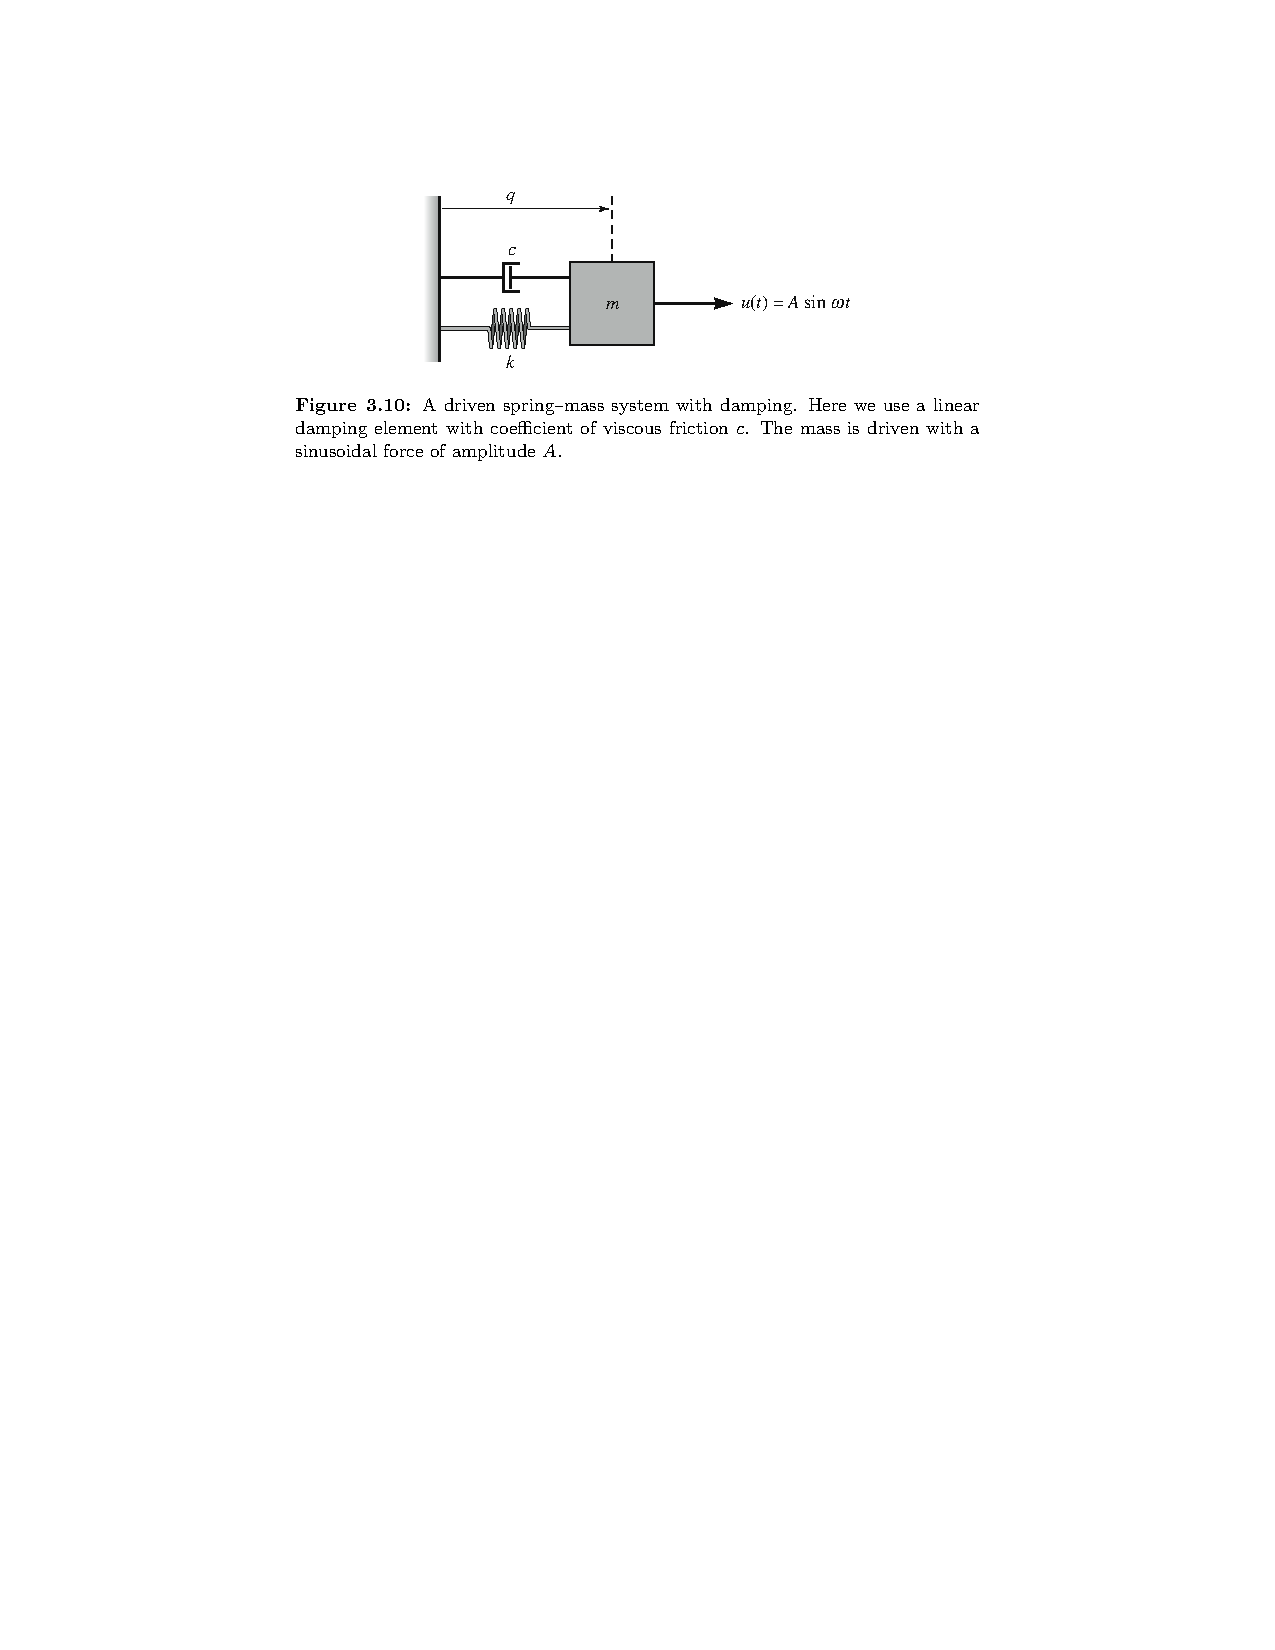
\includegraphics[width=\linewidth]{figure3.10}

Differential form:
\begin{align}
x &= \Matr{q\\\dot q} & \dot x & = \begin{bmatrix}\dot q\\- \frac cm\dot q - \frac km q\end{bmatrix}
\end{align}
$\to$ ODE solver (Matlab, Python)
\end{frame}

\begin{frame}
\frametitle{Simulation --- ODE solvers}
\begin{itemize}
\item Many algorithms for numerically solving ODEs
\item Simulink defaults to \texttt{ode45} with a variable time step solver
\item Important to check solver is accurate -- convergence test(s)
\end{itemize}
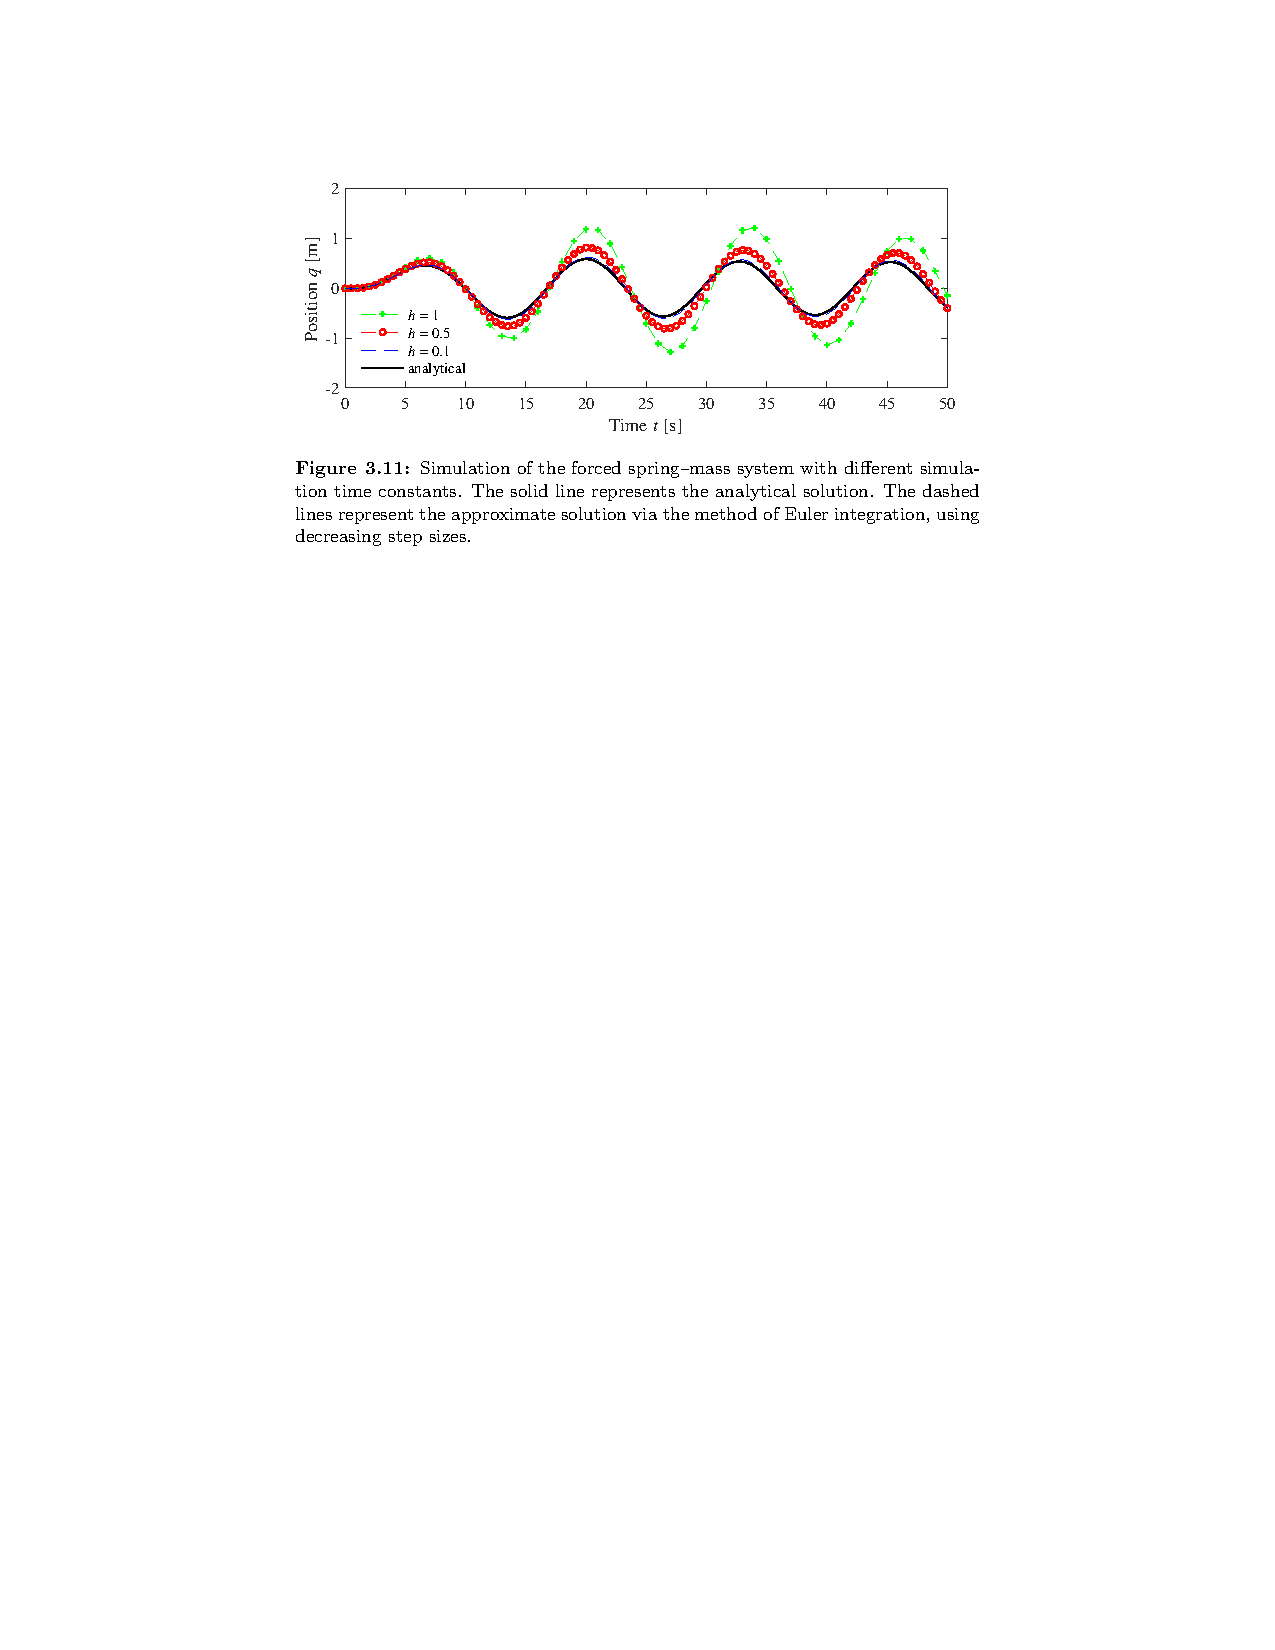
\includegraphics[width=\linewidth]{figure3.11}
\end{frame}

\begin{frame}
\frametitle{Analysis --- stability}
\begin{itemize}
\item
Simulations are great, but we sometimes want to analyse our ODEs meaningfully
\item
Lyapunov stability analysis:
\end{itemize}
\begin{align}
V(x) &= \frac12kx_1^2 + \frac12mx_2^2 & \hspace{5cm}\\
\Deriv{V(x)}{t} &= 
\end{align}
\vfill
\vspace*{1cm}
\begin{itemize}
\item If $\dot V < 0$, the energy of the system is always decreasing, and the system is therefore \dots
\end{itemize}
\vspace*{-1cm}
\end{frame}

\begin{frame}
\frametitle{Analysis --- frequency response}
For a linear time-invariant system such as: (i.e., separable ODE)
\begin{gather}
m\ddot q + c\dot q + k q = u
\end{gather}
We often consider the input/output relationship in terms of sinusoids of given frequency:
\begin{gather}
u(t) = A\sin(\omega t) \\
q(t) = g(\omega)\sin(\omega t + \phi(\omega))
\end{gather}
The frequency response can be derived (see later) or simulated. For nonlinear systems, things get complicated
\end{frame}

\begin{frame}
\frametitle{Analysis --- sketch of a frequency response}
\end{frame}


\SUMMARYFRAME
\FINALE

\end{document}
